% PyQSO User Manual

%    Copyright (C) 2013 Christian Jacobs.

%    This file is part of PyQSO.

%    PyQSO is free software: you can redistribute it and/or modify
%    it under the terms of the GNU General Public License as published by
%    the Free Software Foundation, either version 3 of the License, or
%    (at your option) any later version.
%
%    PyQSO is distributed in the hope that it will be useful,
%    but WITHOUT ANY WARRANTY; without even the implied warranty of
%    MERCHANTABILITY or FITNESS FOR A PARTICULAR PURPOSE.  See the
%    GNU General Public License for more details.
%
%    You should have received a copy of the GNU General Public License
%    along with PyQSO.  If not, see <http://www.gnu.org/licenses/>.

\documentclass[11pt, a4paper]{report}
\usepackage[margin=1.2in]{geometry}
\usepackage{graphicx}
\usepackage{hyperref}
\hypersetup{
  colorlinks=false,
  pdfborder={0 0 0},
  }

\setlength{\parskip}{0.25cm}

\begin{document}

\begin{titlepage}
\begin{center}
\vspace*{5cm}
\huge{PyQSO User Manual}\\\vspace*{5cm}
\LARGE{Version 0.1a}
\end{center}
\end{titlepage}

\tableofcontents

\chapter{Introduction}\label{chap:introduction}
\section{Overview}
PyQSO is a logging tool for amateur radio operators. It provides a simple graphical interface through which users can manage information about the contacts/QSOs they make with other operators on the air. All information is stored in a light-weight SQL database. Other key features include:
\begin{itemize}
  \item Customisable interface (e.g. only show callsign and frequency information).
  \item Import and export logs in ADIF format.
  \item Perform callsign lookups and auto-fill data fields using the qrz.com database.
  \item Sort the logs by individual fields.
  \item Print a hard-copy of logs, or print to PDF.
  \item Connect to Telnet-based DX clusters.
  \item Progress tracker for the DXCC award.
  \item Grey line plotter.
  \item Filter out QSOs based on the callsign field (e.g. only display contacts with callsigns beginning with ``M6'').
  \item Remove duplicate QSOs.
  \item Basic support for the Hamlib library.
\end{itemize}
The source code for PyQSO is available for download at:

\texttt{https://github.com/ctjacobs/pyqso}

\section{Data storage model}
Many amateur radio operators choose to store all the contacts they ever make in a single \textit{logbook}, whereas others keep a separate logbook for each year, for example. Each logbook may be divided up to form multiple distinct \textit{logs}, perhaps one for casual repeater contacts and another for DX'ing. Finally, each log can contain multiple \textit{records}. PyQSO is based around this three-tier model for data storage, going from logbooks at the top to individual records at the bottom. 

Rather than storing each log in a separate file, a single database can hold several logs together; in PyQSO, a database is therefore analogous to a logbook. Within a database the user can create multiple tables which are analogous to the logs. Within each table the user can create/modify/delete records which are analogous to the records in each log.

\section{Licensing}
PyQSO is free software, released under the GNU General Public License. Please see the file called COPYING for more information.

\section{Structure of this manual}
The structure of this manual is as follows. Chapter \ref{chap:getting_started} is all about getting started with PyQSO -- from the installation process through to creating a new logbook (or opening an existing one). Chapter \ref{chap:log_management} explains how to create a log in the logbook, as well as the basic operations that users can perform with existing logs, such as printing, importing from/exporting to ADIF format, and sorting. Chapter \ref{chap:record_management} deals with the bottom layer of the three-tier model -- the creation, deletion, and modification of QSO records in a log. Chapter \ref{chap:toolbox} introduces the PyQSO toolbox which contains three tools that are useful to amateur radio operators: a DX cluster, a grey line plotter, and an awards progress tracker. Finally, Chapter \ref{chap:preferences} explains how users can set up Hamlib support and show/hide various fields in a log, along with several other user preferences that can be set via the Preferences dialog window.

\chapter{Getting started}\label{chap:getting_started}

\section{System requirements}
It is recommended that users run PyQSO on the Linux operating system, since all development and testing of PyQSO takes place there.

As the name suggests, PyQSO is written primarily in the Python programming language. The graphical user interface has been built using the GTK+ library through the PyGObject bindings. PyQSO also uses an SQLite embedded database to manage all the contacts an amateur radio operator makes. Users must therefore make sure that the Python interpreter and any additional software dependencies are satisfied before PyQSO can be run successfully. The list of software packages that PyQSO depends on is provided in the README file.

\section{Installation and running}
Assuming that the current working directory is PyQSO's base directory (the directory that the Makefile is in), PyQSO can be installed via the terminal with the following command:

  \texttt{make install}

\noindent Note: `sudo' may be needed for this. Once installed, the following command will run PyQSO:

  \texttt{pyqso}

\noindent Alternatively, PyQSO can be run (without installing) with:

  \texttt{python bin/pyqso}

\noindent from PyQSO's base directory.

\subsection{Command-line options}
There are several options available when executing PyQSO from the command-line.

\subsubsection{Open a specified logbook file}
In addition to being able to open a new or existing logbook through the graphical interface, users can also specify a logbook file to open at the command line with the \texttt{-l} or \texttt{--logbook} option. For example, to open a logbook file called \texttt{mylogbook.db}, use the following command:

  \texttt{pyqso --logbook /path/to/mylogbook.db}

\noindent If the file does not already exist, PyQSO will create it.

\subsubsection{Debugging mode}
Running PyQSO with the \texttt{-d} or \texttt{--debug} flag enables the debugging mode:

  \texttt{pyqso --debug}

\noindent All debugging-related messages are written to a file called pyqso.debug, located in the current working directory.

\section{Opening a new or existing logbook}
Logbooks are SQL databases, and as such they are accessed with a database connection. To create a connection and open the logbook, click \texttt{Open a New or Existing Logbook...} in the \texttt{Logbook} menu, and either:
\begin{itemize}
  \item Find and select an existing logbook database file (which usually has a \texttt{.db} file extension), and click \texttt{Open} to create the database connection; or
  \item Create a new database by entering a (non-existing) file name and clicking \texttt{Open}. The logbook database file (and a connection to it) will then be created automatically.
\end{itemize}
Once the database connection has been established, the database file name will appear in the status bar. All logs in the logbook will be opened automatically, and the interface will look something like the one shown in Figure \ref{fig:log_view_with_awards}.

\begin{figure}
  \centering
  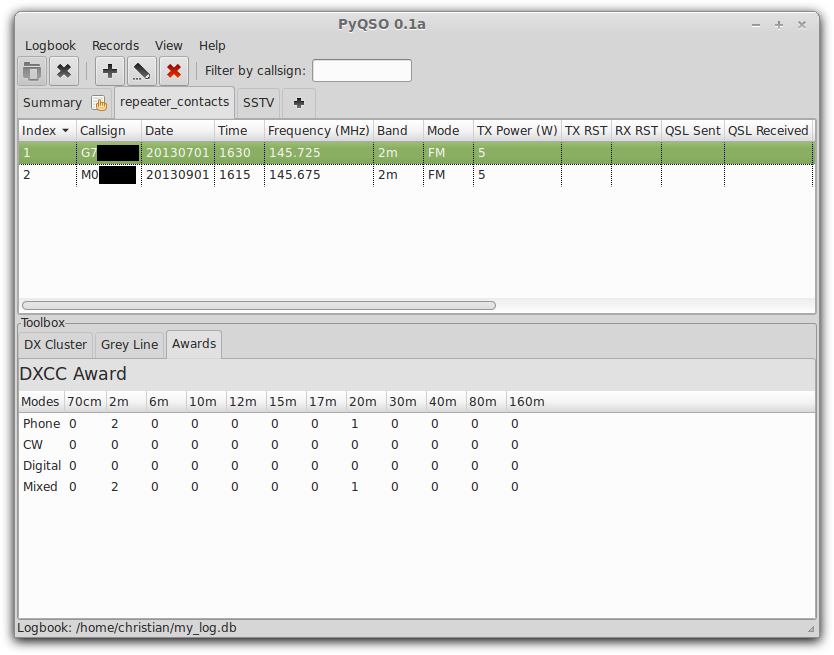
\includegraphics[width=1\columnwidth]{images/log_with_awards.png}
  \caption{The PyQSO main window, showing the records in a log called \texttt{repeater\_contacts}, and the awards tool in the toolbox below it.}
  \label{fig:log_view_with_awards}
\end{figure}

\section{Closing a logbook}
A logbook can be closed (along with its corresponding database connection) by clicking the \texttt{Close Logbook} button in the toolbar, or by clicking \texttt{Close Logbook} in the \texttt{Logbook} menu.

\chapter{Log management}\label{chap:log_management}
\noindent\textbf{Note 1:} All the operations described below assume that a logbook is already open.

\noindent\textbf{Note 2:} Any modifications made to the logs are permanent. Users should make sure they keep up-to-date backups.

\section{Creating a new log}
To create a new log, click \texttt{New Log} in the \texttt{Logbook} menu and enter the desired name of the log (e.g. repeater\_contacts, dx, mobile\_log). Alternatively, use the shortcut key combination \texttt{Ctrl + N}. 

The log name must be unique (i.e. it cannot already exist in the logbook). Furthermore, it can only be composed of alphanumeric characters and the underscore character, and the first character in the name must not be a number. 

Note: When logs are stored in the database file, field/column names from the ADIF standard are used. However, please note that only the following subset of all the ADIF fields is considered: CALL, QSO\_DATE, TIME\_ON, FREQ, BAND, MODE, TX\_PWR, RST\_SENT, RST\_RCVD, QSL\_SENT, QSL\_RCVD, NOTES, NAME, ADDRESS, STATE, COUNTRY, DXCC, CQZ, ITUZ, IOTA.

\section{Renaming a log}
To rename the currently selected log, click \texttt{Rename Selected Log} in the \texttt{Logbook} menu. Remember that the log's new name cannot be the same as another log in the logbook.

\section{Deleting a log}
To delete the currently selected log, click \texttt{Delete Selected Log} in the \texttt{Logbook} menu. As with all database operations in PyQSO, this is permanent and cannot be undone.

\section{Importing and exporting a log}
While PyQSO stores logbooks in SQL format, it is possible to export individual logs in the well-known ADIF format. Select the log to export, and click \texttt{Export Log} in the \texttt{Logbook} menu.

Similarly, records can be imported from an ADIF file. Upon importing, users can choose to store the records in a new log, or append them to an existing log in the logbook. To import, click \texttt{Import Log} in the \texttt{Logbook} menu.

Note that all data must conform to the ADIF standard, otherwise it will be ignored.

\section{Printing a log}
Due to restrictions on the page width, only a selection of field names will be printed: callsign, date, time, frequency, and mode.

\section{Filtering by callsign}
Entering an expression such as \texttt{xyz} into the \texttt{Filter by callsign} box will instantly filter out all records whose callsign field does not contain \texttt{xyz}.

\section{Sorting by field}
To sort a log by a particular field name, left-click the column header that contains that field name. By default, it is the \texttt{Index} field that is sorted in ascending order.

\chapter{Record management}\label{chap:record_management}

\noindent\textbf{Note:} Any modifications made to the records are permanent. Users should make sure they keep up-to-date backups.

\section{Creating a new record (QSO)}
A new QSO can be added by either:
\begin{itemize}
  \item Clicking the \texttt{Add Record} button in the toolbar.
  \item Pressing \texttt{Ctrl + R}.
  \item Clicking \texttt{Add Record...} in the \texttt{Records} menu.
\end{itemize}
A dialog window will appear where details of the QSO can be entered (see Figure \ref{fig:edit_record}). Note that the current date and time are filled in automatically. When ready, click \texttt{OK} to save the changes.

\begin{figure}
  \centering
  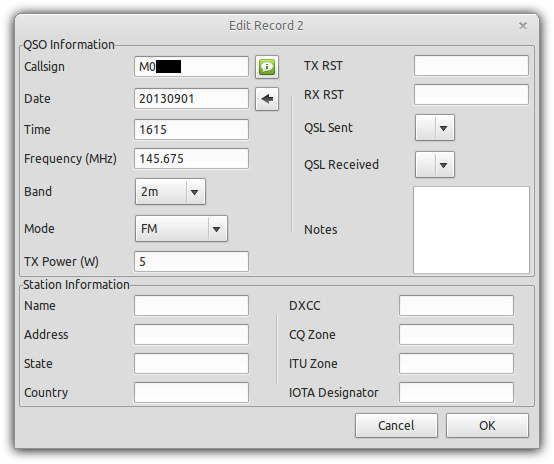
\includegraphics[width=1\columnwidth]{images/edit_record.png}
  \caption{Record dialog used to add new records and edit existing ones.}
  \label{fig:edit_record}
\end{figure}

\subsection{Callsign lookup}
PyQSO can also resolve station-related information (e.g. the operator's name, address, and ITU Zone) by clicking the \texttt{Lookup on qrz.com} button adjacent to the Callsign data entry box. Note that the user must first supply their qrz.com account information in the preferences dialog window.

\section{Editing a record}
An existing record can be edited by:
\begin{itemize}
  \item Double-clicking on it.
  \item Selecting it and clicking the \texttt{Edit Record} button in the toolbar.
  \item Selecting it and clicking \texttt{Edit Selected Record...} in the \texttt{Records} menu.
\end{itemize}
This will bring up the same dialog window as before.

\section{Deleting a record}
An existing record can be deleted by:
\begin{itemize}
  \item Selecting it and clicking the \texttt{Delete Record} button in the toolbar.
  \item Selecting it and pressing the \texttt{Delete} key.
  \item Selecting it and clicking \texttt{Delete Selected Record...} in the \texttt{Records} menu.
\end{itemize}

\section{Removing duplicate records}
PyQSO can find and delete duplicate records in a log. A record is a duplicate of another if its data in the Callsign, Date, Time, Frequency, and Mode fields are the same. Click \texttt{Remove Duplicate Records} in the \texttt{Records} menu.

\chapter{Toolbox}\label{chap:toolbox}
The toolbox is hidden by default. To show it, click \texttt{Toolbox} in the \texttt{View} menu.

\section{DX cluster}
A DX cluster is essentially a server through which amateur radio operators can report and receive updates about QSOs that are in progress across the bands. PyQSO is able to connect to a DX cluster that operates using the Telnet protocol to provide a text-based alert service. As a result of the many different Telnet-based software products that DX clusters run, PyQSO currently outputs the raw data received from the DX cluster rather than trying to parse it in some way.

Click on the \texttt{Connect to Telnet Server} button and enter the DX server details in the dialog that appears. If no port is specified, PyQSO will use the default value of 23. A username and password may also need to be supplied. Once connected, the server output will appear in the DX cluster frame (see Figure \ref{fig:dx_cluster}). A command can also be sent to the server by typing it into the entry box and clicking the adjacent \texttt{Send Command} button.

\begin{figure}
  \centering
  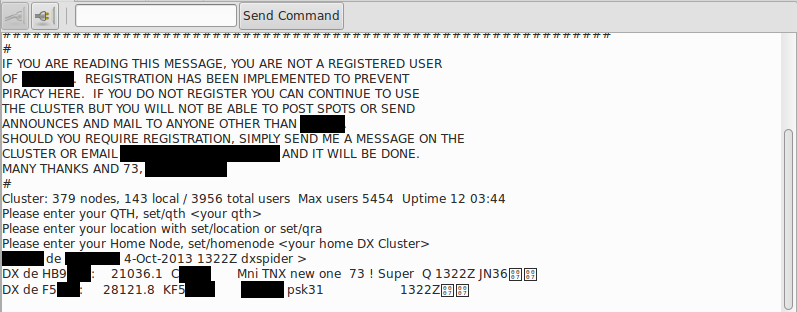
\includegraphics[width=1\columnwidth]{images/dx_cluster.png}
  \caption{The DX cluster frame.}
  \label{fig:dx_cluster}
\end{figure}

\section{Grey line}
The grey line tool (see Figure \ref{fig:grey_line}) can be used to check which parts of the world are in darkness. The position of the grey line is automatically updated every 30 minutes.

\begin{figure}
  \centering
  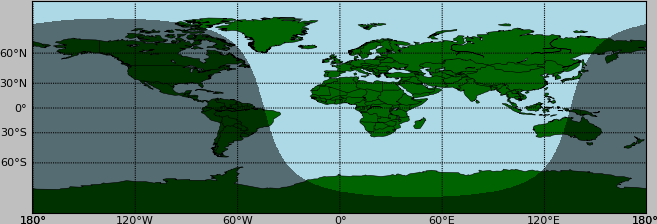
\includegraphics[width=1\columnwidth]{images/grey_line.png}
  \caption{The grey line tool.}
  \label{fig:grey_line}
\end{figure}

\section{Awards}
The awards data is updated each time a record is added, deleted, or modified. Currently only the DXCC award is supported (see Figure \ref{fig:awards}).

\begin{figure}
  \centering
  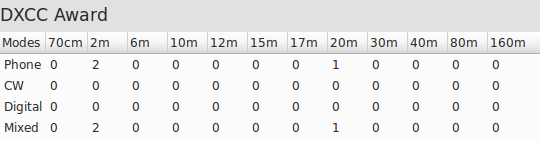
\includegraphics[width=1\columnwidth]{images/awards.png}
  \caption{The award progress tracker.}
  \label{fig:awards}
\end{figure}

\chapter{Preferences}\label{chap:preferences}
PyQSO user preferences are stored in a configuration file located at \texttt{\textasciitilde/.pyqso.ini}, where \texttt{\textasciitilde} denotes the user's home directory.

\section{General}
Under the \texttt{General} tab, the user can choose to show the toolbox (see Chapter \ref{chap:toolbox}) when PyQSO is started.

The user can also enter their login details to access the qrz.com database. Note that these details are currently stored in plain text (unencrypted) format.

\section{View}
Not all the available fields have to be displayed in the logbook. The user can choose to hide a subset of them by unchecking them in the \texttt{View} tab. PyQSO must be restarted in order for any changes to take effect.

\section{Hamlib support}\label{sect:hamlib}
PyQSO features rudimentary support for the Hamlib library. The name and path of the radio device connected to the user's computer can be specified in the \texttt{Hamlib} tab of the preferences dialog. Upon adding a new record to the log, PyQSO will use Hamlib to retrieve the current frequency that the radio device is set to and automatically fill in the Frequency field.

\bibliographystyle{plainnat}
\end{document}
